\item \points{2b} \textbf{Coding problem: The naive method on partial labels}

We now consider the case where the $t$-labels are unavailable, so you only have
access to the $y$-labels at training time. Extend your code in
\texttt{src-incomplete/submission.py} to re-train the classifier (still using $x_1$ and
$x_2$ as input features), but using the $y$-labels only. More specifically, you will implement
the |naive_partial_labels_predictions| function. Output the predictions
on the \textbf{test set} to the appropriate file (as described in the code comments).

Note that the algorithm should learn a function $h(\cdot)$ that approximately predicts the probability $p(y^{(i)}=1\mid x^{(i)})$. Also note that we expect it to perform poorly on predicting the probability of interest, namely $p(t^{(i)}=1\mid x^{(i)})$.

The output plot should look similar to the following (no plot submission is required):
\begin{figure}[H]
	\centering
	\vspace{2mm}
	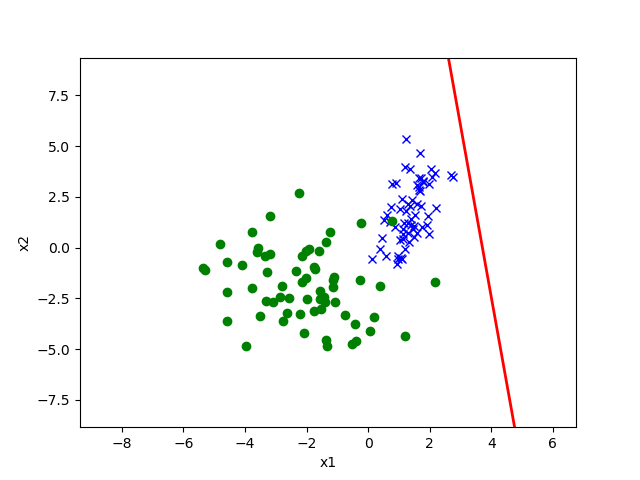
\includegraphics[width=0.5\linewidth]{02-posonly/posonly_naive_pred.png}
    \caption{Separating hyperplane for logistic regression on training set using naive partially observed labels. Visual impaired students can access the corresponding desmos plot \href{https://www.desmos.com/calculator/z7hz6em1by}{here} (Note: This is for reference only.  You are not required to submit a plot.)}
\end{figure}

